\documentclass{beamer}

\usepackage[T1]{fontenc}
\usepackage[utf8]{inputenc}
\usepackage{multirow}

% There are many different themes available for Beamer. A comprehensive
% list with examples is given here:
% http://deic.uab.es/~iblanes/beamer_gallery/index_by_theme.html
% You can uncomment the themes below if you would like to use a different
% one:
%\usetheme{AnnArbor}
%\usetheme{Antibes}
%\usetheme{Bergen}
%\usetheme{Berkeley}
%\usetheme{Berlin}
%\usetheme{Boadilla}
%\usetheme{boxes}
%\usetheme{CambridgeUS}
%\usetheme{Copenhagen}
%\usetheme{Darmstadt}
%\usetheme{default}
%\usetheme{Frankfurt}
\usetheme{Goettingen}
%\usetheme{Hannover}
%\usetheme{Ilmenau}
%\usetheme{JuanLesPins}
%\usetheme{Luebeck}
%\usetheme{Madrid}
%\usetheme{Malmoe}
%\usetheme{Marburg}
%\usetheme{Montpellier}
%\usetheme{PaloAlto}
%\usetheme{Pittsburgh}
%\usetheme{Rochester}
%\usetheme{Singapore}
%\usetheme{Szeged}
%\usetheme{Warsaw}

\title{Web aplikacija za upravljanje rasporedom aktivnosti}

% A subtitle is optional and this may be deleted
%\subtitle{Optional Subtitle}

\author{Juraj Juričić}
% \author{F.~Author\inst{1} \and S.~Another\inst{2}}
% - Give the names in the same order as the appear in the paper.
% - Use the \inst{?} command only if the authors have different
%   affiliation.

\institute[Universities of Somewhere and Elsewhere] % (optional, but mostly needed)
{
  Fakultet elektrotehnike i računarstva\\
  Sveučilište u Zagrebu
}
% - Use the \inst command only if there are several affiliations.
% - Keep it simple, no one is interested in your street address.

\date{Zagreb, srpanj 2017}
% - Either use conference name or its abbreviation.
% - Not really informative to the audience, more for people (including
%   yourself) who are reading the slides online

%\subject{Theoretical Computer Science}
% This is only inserted into the PDF information catalog. Can be left
% out. 

% If you have a file called "university-logo-filename.xxx", where xxx
% is a graphic format that can be processed by latex or pdflatex,
% resp., then you can add a logo as follows:

% \pgfdeclareimage[height=0.5cm]{university-logo}{university-logo-filename}
% \logo{\pgfuseimage{university-logo}}

% Delete this, if you do not want the table of contents to pop up at
% the beginning of each subsection:
%\AtBeginSubsection[]
%{
%  \begin{frame}<beamer>{Outline}
%  \tableofcontents[currentsection,currentsubsection]
%  \end{frame}
%}

% Let's get started
\begin{document}

\begin{frame}
  \titlepage
\end{frame}

\begin{frame}{Sadržaj}
  \tableofcontents
  % You might wish to add the option [pausesections]
\end{frame}

% Section and subsections will appear in the presentation overview
% and table of contents.
\section{Raspoređivanje aktivnosti}

\subsection{Opis problema}

\begin{frame}{Problem raspoređivanja aktivnosti}
  \begin{block}{Zadatak:}
    Složiti (generirati) \textit{dobar} raspored danih aktivnosti pritom pazeći na određena ograničenja.
  \end{block}
    
  \begin{itemize}
    \item {Univerzalna definicija \textit{dobrog} rasporeda \textbf{ne postoji}}
    \item {Velik broj mogućih kombinacija -- kombinatorna eksplozija}
    \item {$\mathcal{NP}$-težak problem}
    \item {Može se svesti na optimizacijski problem -- rješavanje metaheuristikama}
  \end{itemize}
\end{frame}

\subsection{Parametri rasporeda}

\begin{frame}{Parametri rasporeda}
  \begin{itemize}
    \item {Aktivnosti}
    \begin{itemize}
      \item {Naziv}
      \item {\textbf{Trajanje}}
      \item {\textbf{Rok} (engl. \textit{deadline})}
      \item {Prioritet}
    \end{itemize}
    
    \item{Fiksni događaji}
  
    \item{Parametri funkcija dobrote -- \textit{što je dobar raspored?}}
  \end{itemize}
\end{frame}

\subsection{Ograničenja}

\begin{frame}{Ograničenja (engl. \textit{constraints})}
  \begin{itemize}
    \item {Tvrda ograničenja:}
    \begin{itemize}
      \item {Aktivnosti i događaji se \textbf{ne smiju} \textit{preklapati}}
    \end{itemize}
  \end{itemize}
  
  \begin{itemize}
    \item {Meka ograničenja:}
    \begin{itemize}
      \item {Poštivanje roka}
      \item {Poštivanje prioriteta}
    \end{itemize}
  \end{itemize}
\end{frame}

\section{Optimizacijski problem}

\subsection{Funkcija dobrote}
\begin{frame}{Funkcija dobrote (engl. \textit{fitness function})}
  \begin{itemize}
    \item {Funkcija dobrote -- evaluira pojedino rješenje}
    \item {Linearna kombinacija parcijalnih evaluacijskih funkcija}
    
    \begin{itemize}
      \item {Neprekinutost aktivnosti}
      \item {Poštivanje roka}
      \item {Poštivanje prioriteta}
    \end{itemize}
  \end{itemize}
\end{frame}

\section{Web sučelje aplikacije}

\subsection{Unos parametara}

\begin{frame}{Web sučelje aplikacije}{Unos parametara}
\centering
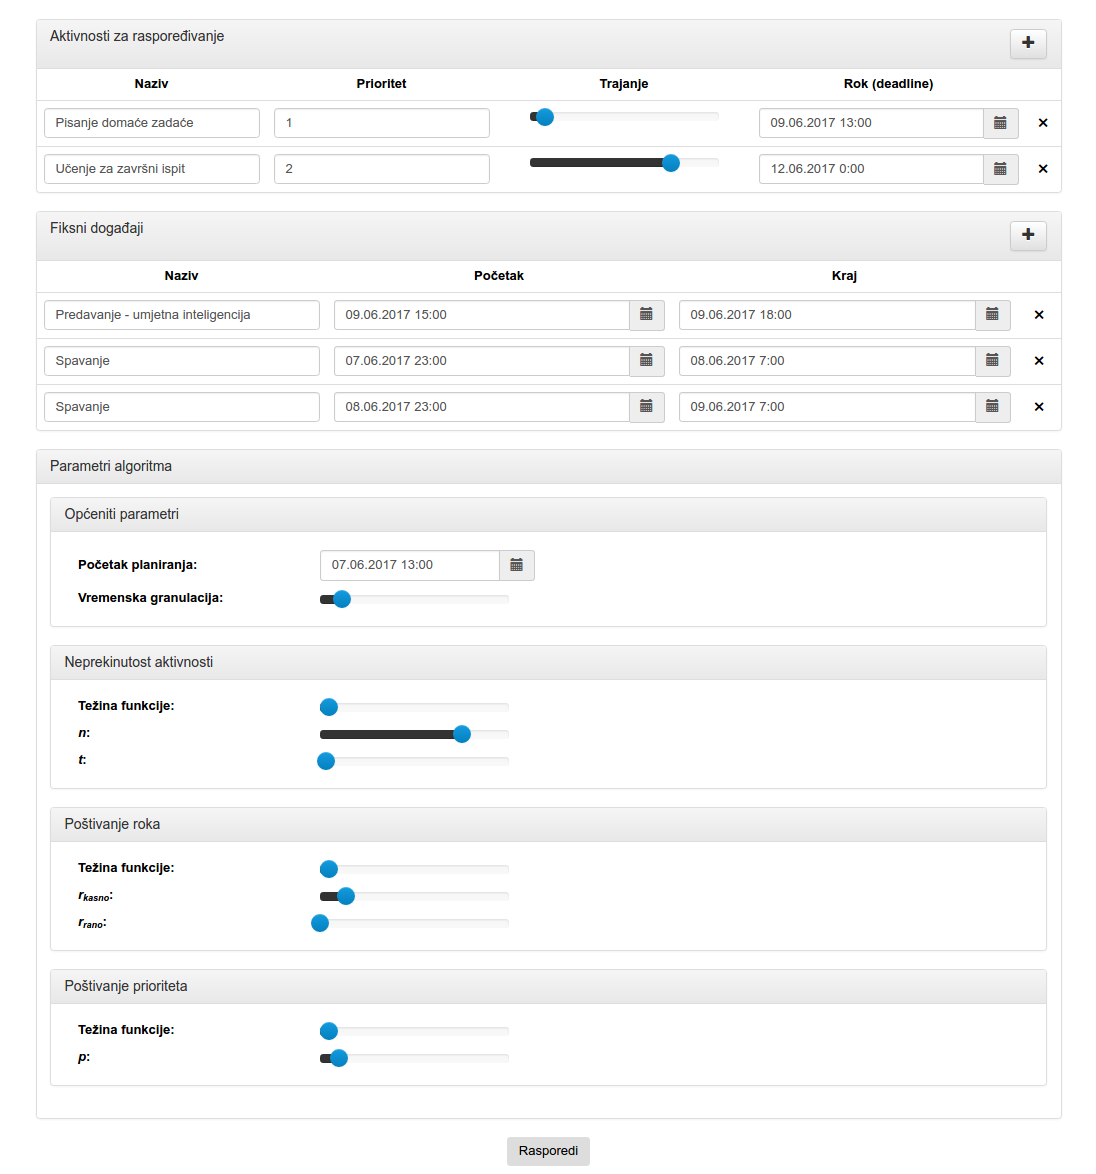
\includegraphics[totalheight=0.8\textheight]{../TeX/resources/graphics/screenshot-form.png}
\end{frame}

\subsection{Generirani raspored}

\begin{frame}{Web sučelje aplikacije}{Generirani raspored}
\centering
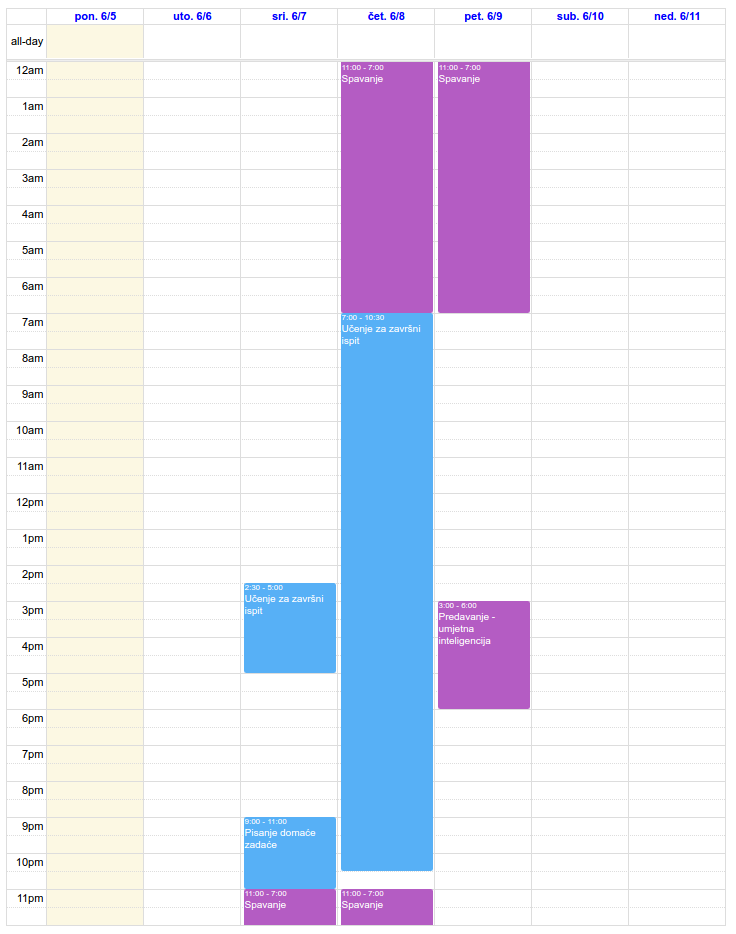
\includegraphics[totalheight=0.8\textheight]{../TeX/resources/graphics/screenshot-raspored-1.png}
\end{frame}

% Placing a * after \section means it will not show in the
% outline or table of contents.
\section*{Zaključak}

\begin{frame}{Zaključak}
  \begin{itemize}
    \item
      Problem raspoređivanja aktivnosti je optimizacijski problem.
      
    \item
      Genetski algoritam se dobro nosi s teškim problemima raspoređivanja aktivnosti.
  \end{itemize}
  
  \begin{itemize}
    \item
      Daljnji rad
    \begin{itemize}
      \item
        Unaprijeđenje web sučelja
      \item
        Učenje navika, praćenje želja korisnika
      \item
        Integracija s drugim alatima, npr. \textit{Google Kalendar} i \textit{Trello}
    \end{itemize}
  \end{itemize}
\end{frame}

\end{document}
